
% !TEX root = ../main.tex

% Local Variables:
% TeX-master: "../main"
% End:
% chktex-file 26

%%%%%%%%%%%%%%%%%%%%%%%%%%%%%%% Header %%%%%%%%%%%%%%%%%%%%%%%%%%%%%%%%%%%%%%%%%%%%
\begin{minipage}[l]{0.42\textwidth}
    \includegraphics[width=1\textwidth]{img/logo-UNAMBA.png}
\end{minipage}
\hfill
\begin{minipage}[c]{0.5\textwidth}
    \begin{flushright}
	\large{\textbf{Unidad \#2}}\\
	\large{Lectures on Física I}\\
	\large{02 de Septiembre del 2025. Haquira, Apurimac}\\
        % \large{\textbf{Student:} Huallpa Aimituma Josué David}
    \end{flushright}
\end{minipage}
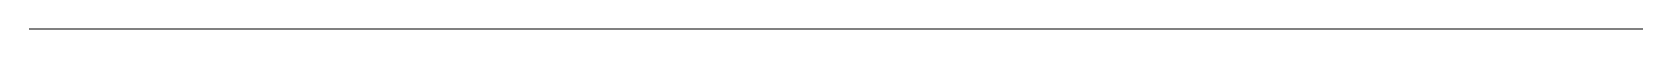
\begin{tikzpicture}
    \draw[gray,thick] (-6.5,0)--(14,0);
\end{tikzpicture}


 %%%%%%%%%%%%%%%%%%%%%%%% INICIO DEL CONTENIDO EN DOS COLUMNAS %%%%%%%%%%%%%%%%%%%%%
  
 \begin{multicols}{2}
   \begin{center}
         \LARGE{\textbf{Capítulo II, III: Vectores -  Estática}}\\	
         \vspace{0.2cm}
         % \Large {Lecturers Esteban Chalbaud \& Daniel Galviz} \\
         % \large{Teaching Assistant: Mauricio Gamonal \& Irvin Martínez}\\
         % \large{PhysicsLatam.com}\\
         % \vspace{0.2cm}
         \large{2 Septiembre 2025, 5:59 pm (GMT-4)}\\
         % \vspace{0.2cm}
         \large{— Sust. Unidad 2 —}
     \end{center}

    \begin{excercise}[][][]{ex:k28-mod}{(\textbf{4 pts})
        Dados los puntos  $P(-6,\,4,\,-3)$, $Q(4,\,-5,\,2)$ y $R(-2,\,-1,\,7)$:  
        \begin{itemize}
            \item[a)] Construir el vector $\vec{v}=\overrightarrow{PR}$.  
            \item[b)] Encontrar la distancia del punto $Q$ a la recta que pasa por $P$ y es paralela al vector $\vec{v}$.  
            \item[c)] Calcular el ángulo formado por los vectores $\vec{QP}$ y $\vec{v}$.  
            \item[d)] Graficar correctamente los puntos $P$, $Q$, $R$, el vector $\vec{v}$, y la recta solicitada en el ítem (b).  
        \end{itemize}
    }
    \end{excercise}

 
    %%%%%%%%%%%%%%%%%%%%%%%%%%%%excercise%%%%%%%%%%%%%%%%%%%%%%%%%%%%%%%%%%%%%%%%
    \begin{excercise}[][][$F_1=F_3=11.5\ \mathrm{lbf} $, $F_2=40\ \mathrm{lgf}$]{ex:32}{ \textbf{(3 pts.)}
        Una escalera AB de peso 40lbf descansa sobre una pared vertical, haciendo un ángulo de $60^\circ$ con el suelo.   
        \begin{figure}[H]
             \centering
             \includegraphics[width=0.7\linewidth]{img/01_physics-i/03_statics/23.png}
         \end{figure}     
        Considerar que todas las superficies son lisas (no hay fuerzas de fricción) y que el peso actua siempre del centro geométrico de la barra. 
        \begin{itemize}
             \item[a)] Encontrar las fuerzas sobre la escalera en A y B. La escalera tiene rodillos en A, de modo que la friccion es despreciable.  
             \item[b)] Resolver el problema usando el método vectorial y escalar para la segunda condición de quilibrio.
         \end{itemize} 
         }
     \end{excercise}

    %%%%%%%%%%%%%%%%%%%%%%%%%%%%excercise%%%%%%%%%%%%%%%%%%%%%%%%%%%%%%%%%%%%%%%%
    \begin{excercise}[][][b)  $\sum\tau_i=\left[160\sqrt{13}\vec{\imath}+120\sqrt{3}\vec{\jmath}+(12-\frac{12}{\sqrt{13}})\vec{k}\right]20\sqrt{13}$]{ex:k29}{(\textbf{3 pts})
            La figura muestra la fuerza $\vec{F}_1$ y $\vec{F_2}$ aplicada en los vértices del paralelepipedo. Si las fuerzas tienen de norma $F_1=500$ N y $F_2=260$ N y siguen las direcciones con las diagonales. 
         \begin{figure}[H]
             \includegraphics[width=\linewidth]{img/01_physics-i/03_statics/sus-1.png}
         \end{figure} 
         \begin{itemize}
             \item[a)] Calcular el vector resultante
             \item[b)] Hallar en torque total con respecto al vértice $A$ 
             \item[c)] Encontrar los ángulos $\alpha, \beta, \gamma$ que forma el vector torque con cada uno de los ejes x, y, z, y  graficar
         \end{itemize}
         }
    \end{excercise}
     %%%%%%%%%%%%%%%%%%%%%%%%%%%%excercise%%%%%%%%%%%%%%%%%%%%%%%%%%%%%%%%%%%%%%%%
     \begin{excercise}[][][$(a)R=137.2\ \mathrm{N}$, $ \tau=0$, $(b)\ R=187.2\ \mathrm{N}$, $\tau=120\ \mathrm{Nm}$]{ex:7}{ \textbf(3 pts.)
         De la figura mostrada, determinar la fuerza y el torque resultantes con respecto a $\mathcal{O}$ de tres fuerzas, 50 N, 80 N, y 100 N, mutuamente perpendiculares entre sí. (a) Si son concurrentes. (b) Si la linea de acción de la fuerza de 100 N se encuentra a 1.2 m del punto de concurrencia de las otras dos.
         \begin{figure}[H]
             \centering
             \includegraphics[width=\linewidth]{img/01_physics-i/03_statics/3.png}
         \end{figure}
         }
     \end{excercise}


\end{multicols}
